\section{Example of symmetry affecting evaluation of electron paths}
In the main text we described the challenges of how to evaluate our model, as different electron paths can form the same products, for instance due to symmetry.
Figure \ref{fig:symmetric-reaction-example} is an example of this.


\begin{figure*}[h]

    \centering
    \begin{subfigure}[b]{0.95\textwidth}
        \centering
        \includegraphics[width=\textwidth]{imgs/symmetry/main_reaction}
        \caption{Reaction as defined by USPTO SMILES}
    \end{subfigure}
    
    \par\bigskip % force a bit of vertical whitespace 
    \begin{subfigure}[b]{0.95\textwidth}
        \centering
        \includegraphics[width=0.4\textwidth]{imgs/symmetry/possible1}
        \qquad
        \qquad
        \includegraphics[width=0.4\textwidth]{imgs/symmetry/possible2}
        \caption{Possible action sequences that all result in same major product.}
    \end{subfigure}
    \caption{This example shows how symmetry can affect the evaluation of electron paths. In this example, although one electron path is given in the USPTO dataset, the initial N that reacts could be either 15 or 12, with no difference in the final product. This is why judging purely based on electron path accuracy can sometimes be misleading.}
    \label{fig:symmetric-reaction-example}
\end{figure*}

\section{Forming Node and Graph Embeddings}

In this section we briefly review existing work for forming node and graph embeddings, as well as describing more specific details relating to our particular implementation of these methods. 
Figure \ref{fig:graph_nn} provides a visualization of these techniques.

\begin{figure*}
\centering
\includegraphics[width=\textwidth]{imgs/graph_nn}
\caption{
Visualization of how node embeddings and graph embeddings are formed. 
Node embeddings are $d$-dimensional vectors, one for each node. 
They are obtained using Gated Graph Neural Networks \citep{li2016gated}.
These networks consist of a series of iterative steps where the embeddings for each node is updated using the node's previous embedding and a message from its neighbors.
 Graph embeddings are $q$-dimensional vectors, representing a set of nodes, which could for instance be all the nodes in a particular graph \citep{li2018learning}.
  They are formed by a weighted sum over node embeddings.
}
\label{fig:graph_nn}
\end{figure*}

 We start with Gated Graph Neural Networks \citep{li2016gated, gilmer2017neural}. 
 We denote these as $\fEmbed: \moleculeSet \to \mathbb{R}^{|\Ac|\times d}$, where we refer to the output as ``node embeddings'', $\nodeEmbeddings{\moleculeSet} \subseteq \mathbb{R}^{|\Ac|\times d}$. 
These networks form these node embeddings through a recurrent operation on messages, $\mb_v$, with $v \in \Ac$ so that there is one message associated with each node.
At the first time step these messages, $\mb_v^{(0)}$, are initialized with the respective atom features shown in Table \ref{table:atom-features}. GGNNs then update these messages in a recursive nature:

\begin{align}
	\mb_v^{(s)} = \textrm{GRU}\left( 
					\mb_v^{(s - 1)},  
						\sum_{i \in \neigh{1}(v)} f_\textrm{single}\left(\mb_i^{(s - 1)}\right) +
						\sum_{j \in \neigh{2}(v)} f_\textrm{double}\left(\mb_j^{(s - 1)}\right) +
						\sum_{k \in \neigh{3}(v)} f_\textrm{triple}\left(\mb_j^{(s - 1)}\right)
					\right)
\end{align}

Where $\textrm{GRU}$ is a Gated Recurrent Unit \citep{Cho2014-xt}, the functions $\neigh{1}(v)$, $\neigh{2}(v)$, $\neigh{3}(v)$ index the nodes connected by single, double and triple bonds to node $v$ respectively and $f_\textrm{single}$, $f_\textrm{double}$ and $f_\textrm{triple}$ are linear transformations with learnable parameters.
This process continues for $S$ steps (where we choose $S=4$), with all the messages and the hidden layer of the GRU maintaining the same dimensionality of 101 as the raw atom features.
The node embeddings are set as the final message belonging to a node, so that indexing a row of the node embeddings matrix, $\nodeEmbeddings{\moleculeSet}$, gives a transpose of the final message vector, ie $[\nodeEmbeddings{\moleculeSet}]_v = \mb_v^{(S)t}$.

\begin{table}
  \caption{Atom features we sue as input to the GGNN. These are calculated using RDKit.}
  \label{table:atom-features}
  \centering
  \begin{tabular}{ll}
    \toprule
    Feature     & Description      \\
    \midrule
    Atom type & 72 possible elements in total, one hot  \\
    Degree     & One hot (0,   1,   2,   3,   4,   5,   6,   7,  10)  \\
    Explicit Valence     & One hot   (0,   1,   2,   3,   4,   5,   6,   7,   8,  10,  12,  14)    \\
    Hybridization & One hot (SP, SP2, SP3, Other) \\
    H count & integer \\
    Electronegativity & float \\
    Atomic number & integer \\
    Part of an aromatic ring & boolean\\
    \bottomrule
  \end{tabular}
\end{table}


Having formed node embeddings we can use these to form graph embeddings \citep{li2018learning,Johnson2017-pd}, which as described earlier are $q$-dimensional vectors representing a set of nodes; i.e.\ an entire molecule or set of molecules.
 We define the function that maps node features belonging to each atom to their graph embedding by $\fEmbedGraphs$.
These are similar to the readout functions used for regressing on graphs detailed in \citep[Eq. 3]{gilmer2017neural} and the graph embeddings described in \citet[\S B.1]{li2018learning}. 
Specifically, $\fEmbedGraphs$ consists of three functions, $\fui$, $\fuj$ and $\fuk$, which could be any multi-layer perceptron (MLP) but in practice we find that linear functions suffice.
They are used to form the graph embedding, as
\begin{align}
	\fEmbedGraphs(\nodeEmbeddings{\moleculeSet_t}) = \fuk\left(\sum_{v \in \Ac'} \sigma\left(\fui(\nodeEmbeddings{\moleculeSet_t,v})\right) \fuj(\nodeEmbeddings{\moleculeSet_t, v})\right).
	\label{eq:graph-embedding}
\end{align}
Where $\sigma$ is a sigmoid function.
We can break this equation down into two stages.
In stage (i), similar to \citet[\S B.1]{li2018learning}, we form an embedding of one or more molecules (with vertices $\Ac'$ and with $\Ac' \subseteq  \Ac$) by performing a gated sum over the node features. 
In this manner the function $\fui$ is used to decide how much that node should contribute towards the embedding,
 and $\fuj$ projects the node embedding up to a higher dimensional space; following \citet[\S B.1]{li2018learning}, we choose this to be double the dimension of the node features.
Having formed this embedding of the graphs, we project this down to a lower $q$-dimensional space in stage (ii), which is done by the function $\fuk$. 







\section{More training details}

In this section we go through more specific model architecture details omitted from the main text. 

\subsection{Model architectures}
In this section we provide further details of our model architectures.

Section 3 of the main paper discusses our model.
In particular we are interested in computing three conditional probability terms: (1) $p_\theta(a_0 \mid \initialAndReactants)$, the probability of the initial state $a_0$ given the reactants and reagents; 
(2) the conditional probability $p_\theta(a_t \mid \moleculeSet_t, a_{t-1}, t)$  
of next state $a_t$ given the intermediate products $\moleculeSet_t$ for $t > 0$;
and (3) the probability $p_\theta(s_t \mid \moleculeSet_t)$ that the reaction terminates with final product $\moleculeSet_{t}$.

Each of these is parametrized by NNs. We can split up the components of these NNs into a series of modules, all introduced in the main text: $\fEmbedGraphs_{\textrm{stop}}$, $\fEmbedGraphs_\mathrm{reagent}$, $\fAdd$, $\fRemove$ and $\fInitial$.
 In this section we shall go through each of these in turn.




As mentioned above  both $\fEmbedGraphs_{\textrm{stop}}$, $\fEmbedGraphs_\mathrm{reagent}$ consist of three
linear functions. 
For  both, the function $\fui$ is used to decide how much each node should contribute towards the embedding and so projects down to a scalar value.
Again for both, $\fuj$ projects the node embedding up to a higher dimensional space, which we choose to be 202 dimensions. 
This is double the dimension of the node features, and similar to the approach taken by \citet[\S B.1]{li2018learning}.
Finally, $\fuk$ differs between the two modules, as for $\fEmbedGraphs_{\textrm{stop}}$ it projects down to one dimension (to later go through a sigmoid function and compute a stop probability), whereas for  $\fEmbedGraphs_\mathrm{reagent}$, $\fuk$ projects  to a dimensionality of 100 to form the reagent embedding.


The modules for $\fAdd$ and $\fRemove$, that operate on each node to produce a action logit, are both NNs consisting of one hidden layer of 100 units. 
Concatenated onto the node features going into these networks are the node features belonging to the previous atom on the path.



The final function, $\fInitial$, is represented by an NN with hidden layers of 100 units. 
When conditioning on reagents (ie for
 \ourModelR
 )
  the reagent embeddings calculated by $\fReagEmbed$ are concatenated onto the node embeddings and we use two hidden layers for our NN. When ignoring reagents (ie for \ourModelIR) we use one hidden layer for this network. In total \ourModelR has approximately 250,000 parameters and \ourModelIR has approximately 190,000.

\subsection{Training}

We train everything using Adam \citep{kingma2014adam} and an initial learning rate of 0.0001, which we decay after 5 and 9 epochs by a factor of 0.1. 
We train for a total of 10 epochs.
For training we use reaction minibatch sizes of one, although these can consist of multiple intermediate graphs.



\section{Prediction using our model}

At predict time, as discussed in the main text, we use beam search to find high probable chemically-valid paths from our model. Further details are given in Algorithm~\ref{algo:valid_path}.

\begin{wrapfigure}{R}{0.5\textwidth}
\begin{minipage}{0.5\textwidth}
\begin{algorithm}[H]
  \caption{Mapping to valid paths.}
  {\bf Input:}~~Predicted path $\hat{\Pc} = [\hat{a}_0, \hat{a}_1, \ldots, \hat{a}_{T-1}]$\\
  {\bf Input:}~~Molecule $\Mc_0$, remove flag $\texttt{F}_\textrm{remove} \!=\!1$
  
  \begin{algorithmic}[1]
  	\STATE Sample initial atom $\hat{a}_0 \sim p(a_0 \mid \Mc_0)$.
    \STATE $\hat{\Pc} = [\hat{a}_0]$%\ab^*_0]$
  	%\FORALL{atoms $\ab$ in molecule $\Mc_1$}
    %	\STATE 
    	%\STATE $i^* = \arg\min_{i \in \{1,\ldots,n\}} 
    %\ENDFOR
    \FORALL{$t$ from $1$ to $T-1$}
    	%\STATE Select predicted path $\hat{pb}_t$
    	\IF{$\texttt{F}_\textrm{remove} = 1$}
    		\STATE Sample atom $a \sim p(a_t \mid \hat{a}_{0:t-1}, \Mc_0)$% (or null action $\mathbf{0}$ if $t \neq T-1$) to $\hat{\ab}_t$, such that the bond $(\ab^*_{t-1}, \ab^*_{t})$ \emph{exists} in $\Mc_t$.
            \IF{$a$ is not `null'}
            	\STATE $\texttt{F}_\textrm{remove} = 0$
            \ENDIF
            \STATE Set $\Mc_t$ to molecule $\Mc_{t-1}$ but with bond $(\hat{a}_{t-1}, a)$ removed.
        \ELSE
        	\STATE Sample atom $a \sim p(a_t \mid \hat{a}_{0:t-1}, \Mc_0)$
            \IF{$a$ is not `null'}
            	\STATE $\texttt{F}_\textrm{remove} = 1$
            \ENDIF
            \STATE Set $\Mc_t$ to molecule $\Mc_{t-1}$ but with bond $(\hat{a}_{t-1}, a)$ added.
   		\ENDIF
        \STATE Set $\hat{a}_t = a$
        \STATE $\hat{\Pc} = [\hat{\Pc}, \hat{a}_t]$
    \ENDFOR
  \end{algorithmic}
  {\bf Output:}~~Valid path~$\hat{\Pc}$
  \label{algo:valid_path}
\end{algorithm}
\end{minipage}
\end{wrapfigure}



\newpage
\quad
\newpage

\section{Further example of actions proposed by our model}

Figure \ref{fig:extra-textbook-example} shows the model's predictions for the mechanism of how two molecules will react. 

\begin{figure*}[h]
        \centering
        \includegraphics{imgs/textbook/reactants2}
        \caption{Predicted mechanism of our model on reactant molecules. Green arrow shows preferred mechanism, whereas pink shows the model's second preferred choice. Here, the first-choice prediction is incorrect, but chemically reasonable, as the Weinreb amide is typically used together in reactions with Magnesium species. The second-choice prediction is correct.}
        \label{fig:extra-textbook-example}
\end{figure*}

\begin{figure*}[h]
        \centering
        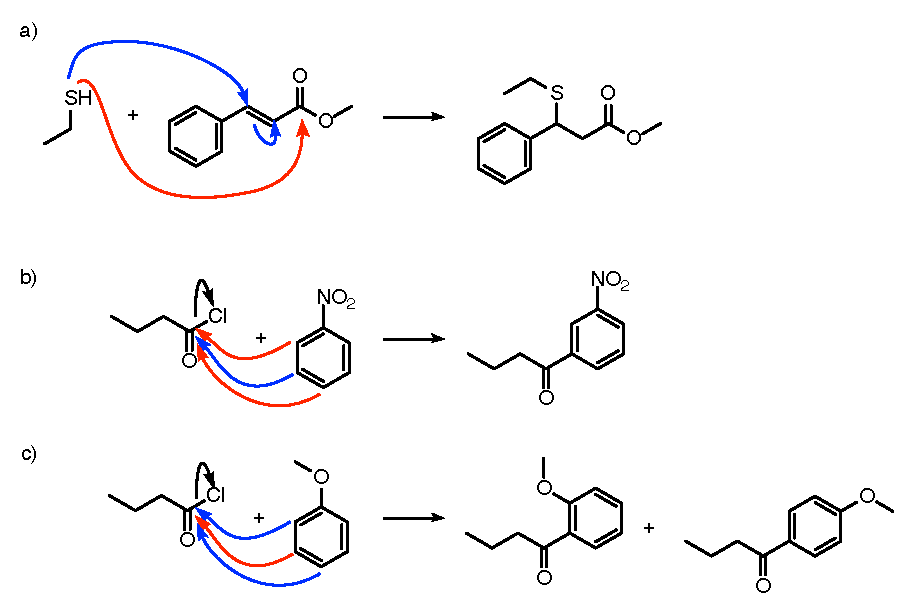
\includegraphics[width=0.7\textwidth]{imgs/textbook/additionalexamples.eps}
        \caption{Additional typical selectivity examples: Here, the expected product is shown on the right. The blue arrows indicate the top ranked paths from our model, the red arrows indicate other possibly competing but incorrect steps, which the model does not predict to be of high probability. In all cases, our model predicted the correct products. In b) and c), our model correctly recovers the regioselectivity expected in electrophilic aromatic substitutions.}
        \label{fig:extra-textbook-example2}
\end{figure*}



